\subsection{Background}
\paragraph{} 
Mr Snowden is a Physics Teacher at Northgate High School, teaching the subject at levels from KS3 to A-Level, there are also several other teachers in the department. During lessons, there are some times where it can be useful to the students to be able to see a model of the subject that they are learning about, while the majority of subjects that are taught have a range of models available, both real and software models. However one of the subjects where models are quite limited is in orbital mechanics and circular motion, with most being just simple animations and not a fully interactive or real-time simulation. The main disadvantage of this is that the students are not able to easily see how different modifications to a system will affect the outcome, something that can help to improve the understanding of a particular topic in some scenarios.

\subsubsection{Project Objective}
\paragraph{}
Mr Snowden requires a teaching tool that can provide a graphical sandbox to create and simulate various scenarios to fortify and replace the currently used tool-set of simple animations and power-point presentations that are used in teaching. This would allow the teacher in a physics lesson to quickly show students how a situation would develop, making use of SI units in order to effectively show students how different parameters (Mass, Size and Velocity) would affect a situation.

\subsubsection{Prospective Users}
\paragraph{}
While Mr Snowden is intended to be the primary user, other teachers could also have access to the tool as it could be put on the shared network drive, making the tool easy to access and used as a teaching aid in lessons, the tool will also be accessed by students, allowing the tool to be used as a revision resource for individual students on the school computers or at home. Because of this special attention should be paid to make sure that the program is as compatible as possible 

\subsection{Requirements and Processes}
\paragraph{}
The interface must be intuitive and self-explanatory in order to ensure that it is easy for teachers to understand, meaning that keyboard short-cuts should be commonly known and any buttons should be clearly labelled. It must also be able to run well on the school computers, most of which are running on low end hardware (Dual-Core HT Intel i3 / Quad-Core Intel i5, ~2-4GB RAM) using a 32-Bit Windows operating system, as this is what all computers in the school are running for internal compatibility reasons. This applies a limit of 4GB to the total system RAM but a maximum per program usage of 2GB, meaning that the program will need to handle memory efficiently and potentially have a limit on the number of bodies (In the range of 1000s) to avoid using too much memory and causing the system to crash, a sensible limit would be 500MB. The number of bodies that this would support can be estimated however actual memory usage will likely be higher due to graphics library overhead, meaning that memory profiling should be used. The program must not require installation on the system or any secondary redistributes to be installed containing dynamic libraries.

\subsubsection{Graphics Processing}

\paragraph{}
While the resources of these systems are limited, keeping the program to being 2D should help to improve performance as there will be less demand on the integrated GPU (Graphics Processing Unit), meaning that it requires less system resources to display the simulation. This means that an external graphics library would need to be used in order to interface with this hardware and still function across different platforms. (The two main GPU Vendors, AMD and Nvidia, both have different interfaces for using GPUs for compute applications) 

\paragraph{}Having a 2D model also means that far less calculations need to be made for the simulation, making it faster, but it also reduces the load GPU in terms of rendering, As 3D would require shading and lighting to make depth perceivable. Input and camera movement would also be far more complex.

\subsubsection{Calculations and Trigonometry}

\paragraph{}
The application must be able to simulate the paths of at least three bodies, as this will encounter the n-body problem (n = Any positive integer), which in essence means that any interaction between two bodies can simply be predicted, however there is no direct solution for three or more bodies, and must be simulated through iterative process between each body to every other body.
The main calculation that will be used between bodies is:

$$F=\frac{Gm_1m_2}{d^2}$$

This calculation produces a result for the gravitational force between objects, taking into account the mass of the two planets and the distance between them, based on a universal gravitational constant. ($\num{6.67408e-11} m^{3} kg^{-1} s^{-2}$) 
While this equation only works between two bodies, the equation can be repeated in an iterative fashion in order to calculate the forces between all bodies in a system, the force can then be resolved to a single dimension for X and Y respectively, and then using a value for mass, acceleration can be calculated. By multiplying the acceleration by the change in time ($\Delta t$) of the simulation you can propagate a velocity ($v$) and change the position ($p$) of a body.

$$F_y=F\sin{\theta} \hspace{20pt} F_x=F\cos{\theta}$$

\paragraph{}
The main issue that could crop up is the computational cost of the trigonometric functions, while the instruction set used by processors in nearly all modern desktop computers (x86) has specific instructions for these functions.
The issue is that these still take longer than simple mathematical operators, which generally only take single instruction cycles. The difficulty is however that it will be heavily dependant both on the particular CPU running the code, but also the compiler used as well as the implementation used by the programming languages libraries.

\paragraph{}
There is also the issue that signs of calculated components to be flipped depending on which quadrant the simulated particle is in, adding further computational complexity. Trigonometric functions are also required to calculate the angle that the force is acting relative to the global X axis.

\paragraph{}
Because of these difficulties, it is worth investigating alternative methods for the calculation of the forces, as there could be far simpler methods that reduce the required complexity of code.

\subsubsection{Performance and Multithreading}

\paragraph{}
\textit{Since the Mid-2000s, CPU Clock speeds have all but stopped increasing in the consumer market, with most coming in at the 2GHz to 3GHz range. Some high end desktop processors are able to be effectively over-clocked, with processors like the AMD FX-9590 capable of 5GHz as long as adequate cooling is provided, the current world record is 8.794GHz, achieved by an AMD FX-8350, however this with with the use of Liquid Nitrogen to keep it cool.}

\paragraph{}
\textit{While clock speeds are effectively limited by the stability that can be achieved in the material being used (Silicon) and thermal properties, the focus has now switched to increasing the core count of CPUs, as well as improving their power efficiency and increasing their transistor count by shrinking the size of the transistors on die. (Consumer Intel CPUs are currently at 14nm, with 10nm on road map for 2017 and 5nm by 2021)}

\paragraph{}
\textit{Most Modern CPUs can be found with a core count of 2 or 4, with technologies such as hyper-threading allowing for multiple threads to be executed per core, effectively increasing the number of 'logical cores' by a factor of 2. High end desktop and workstation CPUs can be found with 6-12 physical cores, allowing for 12-24 consecutive threads. (Server CPUs are now coming with upwards of 18 physical cores, giving them 36 threads. These systems can also support multiple CPUs on the same motherboard, up to 8, allowing for effectively 288 consecutive threads on a single server.)}

\paragraph{}
Mutli-threading leads to is the potential to speed up the execution of the program by computing multiple parts of it at the same time. All of the computers in the school are new enough to have at a minimum dual core Intel i3 with hyper-threading, giving them a total of 4 'logical cores', this means that there is definitely some potential to improve the execution speed of the program.

\paragraph{} 
This opens up new challenges in the form of ensuring that the programming is \textit{'thread safe'}, this means that the program is not going to \textit{‘step on its own toes’}, for example modifying data while another thread is reading it causing lock-ups, or race conditions where one thread completes a task before another and the program fails. When done properly the improvements to performance can be quite impressive.

\subsubsection{Saving of Scenarios}

\paragraph{}
The system will also need the ability to save the current scenario to a file, most likely a plain comma separated value file with a different file extension such as .sav, this will allow a teacher to set up a scenario inside the program outside of lesson time and save it for a future lesson, at which point it can be loaded into the program and used as a quick demo. These files could also be provided to students for use in their revision. Data for every body would need to be stored, namely Mass, Velocity and Position, constants could also be stored which would enable them to be changed in particular scenarios.

\subsubsection{Scale}

\paragraph{}
It is unlikely that true scale would translate particularly well to a program like this without visual aids added to the program, as distances are extremely massive, and planets are extremely small small in comparison to the sun, let alone the distances involved, for example, Earth has a diameter of only 12700 km, however it orbits the sun at a height of 150 Million km. At a zoom where both the sun and earth will be visible, the earth will be too small to make out, even on extremely high resolution monitors.

\subsubsection{Summary: Requirements and Processes}
\begin{itemize}
\item Intuitive and clean interface making use of common keyboard short-cuts.
\item The program must be compatible with as many computers as possible, as it must be able to be run by students outside of school as well as on the school computers. Care must be made to ensure that code is portable and can be easily recompiled for other operating systems, such as Linux or Mac OSX.
\item It must run on 32-bit computers and operating systems.
\item The program must be able to simulate n-bodies, with the only limit being acceptable performance and the amount of memory being used. The body limit will be based on the amount of memory being used. (Max 500MB)
\item The user should be able to set up a scenario to save and then use at a later date.
\item The user will have complete freedom to change to scale the scenario how they please and will be given complete control of constants such as the gravitational constant, as this would make smaller scale simulations more feasible.
\item The program will make use of simple 2D graphics to keep system resource requirements low and boost performance. (3D is not in scope for this project)
\item A graphics library should be used that allows efficient usage of a computer's GPU in order to accelerate the rendering of the simulation.
\item Multi-threading could be investigated in order to improve the performance of simulation and handling of rendering.
\item Some limitations will be required on variables such as position and velocity in order to ensure that a minimum precision is kept and that the laws of physics are not violated. (Speed of Light)
\end{itemize}

\subsection{Data Management}
\subsubsection{Data Sources and Destinations}
\import{tables/}{1_datasrcdest.tex}
% Data Sources and Destinations Table
\paragraph{}
\begin{itemize}
\item Direct user input will be relatively low volume, taken in using keyboard short-cuts and mouse control, the user operates the program in order to place down objects, adjusting the initial size, mass and velocity of bodies in order to set-up the scenario, the user can also stop and start the program and change the speed of time within the simulation as well as other constants.
\item The loading and saving of scenarios will be sending and receiving similar data to what is provided by user inputs, however the data for an entire scenario will be transferred in one go, this includes the mass and size of bodies, as well as the most recent resolved (X, Y), Force, Velocity and Position of each simulated body, various constants that are set should also be stored, such as the gravitational constant, which can be changed by the user.
\item During the running of the simulation, the program will aim to keep the frame-rate (screen update) at 60 frames per second, (Ensures very smooth animation and responsiveness), this means that the data volumes during the running of the simulation are very high, as each frame could be a simulation update, this includes updating the resolved (X, Y) forces, velocity, acceleration and position of each body, according to how much simulation time passed per each frame.
\end{itemize}

\pagebreak

\subsubsection{Data Dictionary}
\paragraph{}
The main flow of data around the program will be body data, as there will need to be a container of some data type that will contain a large number of these bodies. Because this is a simulation, I want to make use of the common double data type, this is the IEEE Standard, 64 bit variable providing anywhere from 15-17 digits of precision depending on the specific hardware and software implementation used.

\paragraph{} 
While a float variable is smaller and only 32-Bits long, it is generally considered that there will be minimal computational benefit from using float instead of double on CPU bound simulations. In the majority of language mathematical functions take in double variables. While these can still take float variables, the operation will still performed as a double variable.

\paragraph{}
The double variable will also be useful for providing extra precision when it comes to the simulation variables, allowing the simulation to be potentially more accurate, however there may be situations where float can be beneficial to the memory footprint of the program.

\paragraph{}
It is also worth noting that if the simulation was being written to run on a GPU, the variables would need to be stored as floats unless a GPU with a large amount of double-precision units was being used as the target, as most GPUs will only have a small number of double-precision cores, often resulting in their performance being lower than what could be achieved using a CPU.

\paragraph{}
The variables written in the table below are likely to change as this project develops, particularly once the specific implementation is picked, things like program flow are more likely to develop during the programming stage.

\import{tables/}{2_datadictionary.tex}
% Data Dictionary Tables

\pagebreak

\subsubsection{Data Flow Diagrams}
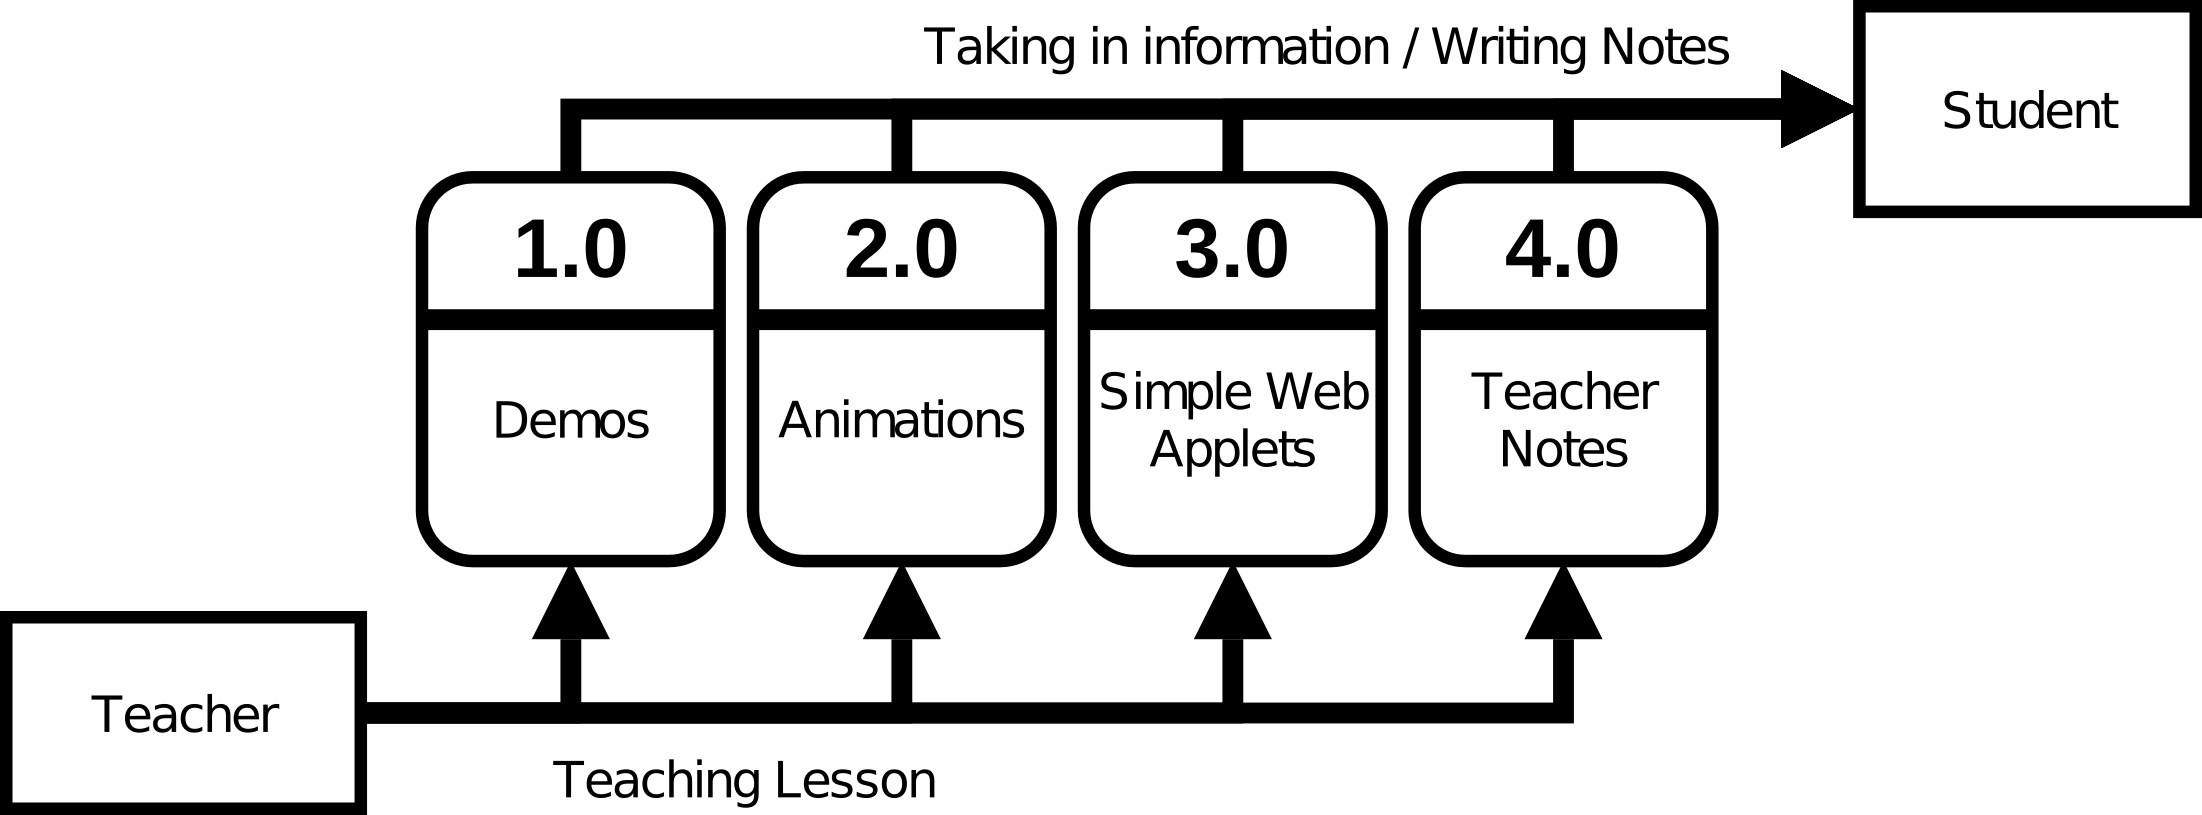
\includegraphics{img/csl1.png}

\subsection{Objectives}

\subsubsection{System}
\begin{itemize}
\item The system must perform well under the kind of scenarios that are likely to need to be demonstrated by a teacher, for A2, this generally does not go over 2 bodies, however having a much larger number of bodies could be useful for showcase simulations.
\item Target performance is 60 frames per second with 100 bodies on screen.
\item The graphics used in the program should be rudimentary 2D vector shapes and lines of varying colours in order to effectively convey the information without becoming too crowded.
\item The program must be compiled to run under 32-bit Windows. it should also not require any external dependencies to be installed in order to run and should be able to be run from any folder on any computer.
\item The size of the scenario should be limited so that objects the precision on the position of the far bodies is not too large, which would potentially affect the simulation.
\end{itemize}


\subsubsection{Processing}
\begin{itemize}
\item The application will use the gravitational force equation to calculate the force between two bodies and newtons second law to convert to acceleration.
\item Trigonometric functions are the currently known way to resolve vector forces to a global X and Y axis. Because of the computational cost these are likely to have an alternative should be investigated.
\item Collisions can be simulated using basic conservation of momentum equation, in order to calculate the resultant direction of travel.
\item The simulation should not be able to take up more than 500MB of system memory, meaning that memory usage must be profiled and a limit coded in.
\item The system should make use of dedicated hardware features such as the GPU to accelerate rendering, this will require external libraries in order to maintain compatibility on multiple computers.
\item Multi-threading should be used to improve runtime performance where it is needed, as well as improve the overall user experience.
\item If multi-threading is used, the programming must be thread safe in order to prevent lock ups or race conditions, each thread must be aware of the state of other threads in order to prevent this.

\end{itemize}

\subsubsection{User}
\begin{itemize}
\item The interface to the program should be basic and self explanatory, making use of the mouse for the placement (position) of bodies and definition of size, mass and velocity, the keyboard can be used for more precise entry of values.
\item It should be possible for the the user to save scenarios that have been set-up so that they can be accessed at a later date or shared with others. The data can be saved to a single file that can be loaded into the program, allowing teachers to set up a scenario outside lesson time to use as a demo.
\item The output of the program should be able to show up well on a projector, meaning that bodies must contrast highly with the background as well as with each other, it may be useful to allow the user to choose the colour of bodies.
\item The user should be able to change any of the values for bodies, position, mass, velocity, should all be possible to change on the fly even when the simulation is running.
\item The user should also be able to change variables such as the gravitational constant and time acceleration to suit smaller scale simulations which will be more visible and understandable to students.
\end{itemize}